% pre2.tex
%
% Purpose:
%   Focused Beamer report on Bloch trace spaces, radiation/admissibility
%   conditions, and DtN-type port conditions for the periodic-lead
%   scattering and eigenvalue formulations in this repository.
%
% Main workflow:
%   The slides isolate the trace-theory chain behind the port formulation:
%   Rayleigh wall coordinates, local homogeneous continuation, one-cell
%   Bloch eigentraces, incoming/outgoing half-lead trace subspaces, and
%   DtN graph interpretations.
%
% Based on:
%   notes/theory/scat_formulation.md, notes/theory/scat_formulation2.md,
%   notes/theory/bloch_mode.md, notes/theory/mode_selection.md,
%   notes/theory/bloch_ode.md, pre/pre1/pre1.tex, and the Joly--Fliss
%   absorbing half-guide perspective referenced by pdf/Joly2006.pdf.
%
% Main differences:
%   Unlike pre1, this file is not a broad TEP/scattering overview.  It is a
%   shorter conceptual deck dedicated to trace spaces and exterior conditions.
%
% Numerical goal:
%   Provide notation and theoretical context for interpreting the Bloch
%   trace matrices and DtN-type port constraints used by the MATLAB
%   experiments.

\documentclass[aspectratio=169]{beamer}

% Theme options:
% \usetheme{CambridgeUS}
% \usetheme{Madrid}
% \usetheme{Boadilla}
\usetheme{CambridgeUS}
\usecolortheme{dove}
\usefonttheme{professionalfonts}

\usepackage{amsmath}
\usepackage{amssymb}
\usepackage{bm}
\usepackage{graphicx}
\usepackage{tikz}
\usepackage{url}
\usetikzlibrary{arrows.meta,positioning}

\newcommand{\ii}{\mathrm{i}}
\newcommand{\Ccell}{\mathcal C}
\newcommand{\Ein}{\mathcal E_{\mathrm{in}}}
\newcommand{\Eout}{\mathcal E_{\mathrm{out}}}
\newcommand{\Din}{D_{\mathrm{in}}}
\newcommand{\Nin}{N_{\mathrm{in}}}
\newcommand{\Dout}{D_{\mathrm{out}}}
\newcommand{\Nout}{N_{\mathrm{out}}}
\newcommand{\tr}{\operatorname{Tr}}
\newcommand{\range}{\operatorname{range}}
\newcommand{\FigurePlaceholder}[1]{%
  \begin{center}
    \setlength{\fboxsep}{1.2em}%
    \fbox{\parbox{0.75\textwidth}{\centering #1}}%
  \end{center}%
}
\newcommand{\SafeIncludeGraphics}[2][]{%
  \IfFileExists{#2}{%
    \includegraphics[#1]{#2}%
  }{%
    \FigurePlaceholder{Missing figure: \url{#2}}%
  }%
}

\title[Bloch Trace Spaces]{Bloch Trace Spaces, Radiation Conditions,\\and DtN-type Port Conditions}
\author{}
\date{}

\AtBeginSection[]{
  \begin{frame}{Outline}
    \tableofcontents[currentsection]
  \end{frame}
}

\begin{document}

\begin{frame}
  \titlepage
\end{frame}

\begin{frame}{Outline}
  \tableofcontents
\end{frame}

\section{Trace Coordinates and Local Rayleigh Continuation}

\begin{frame}{Purpose of This Presentation}
  \begin{itemize}
    \item \texttt{pre1} gives the broad TEP / scattering workflow.
    \item This deck focuses only on trace coordinates, Bloch propagation,
    radiation/admissibility, and DtN-type port conditions.
    \item The goal is to make clear which objects are coordinates, which are
    physical modes, and which are exterior conditions.
  \end{itemize}
  \[
    \boxed{
      \text{Rayleigh coordinates}
      \ne
      \text{Bloch modes}
      \ne
      \text{radiation condition}
      \ne
      \text{DtN map}
    }
  \]
\end{frame}

\begin{frame}{Why Radiation Conditions Matter}
  \small
  An eigenvalue problem is \textbf{not just any nonzero local solution}.
  Local equations alone are too weak:
  \[
    \text{local Helmholtz + transmission}
    \;\not\Rightarrow\;
    \text{eigenmode}.
  \]
  For a single scatterer, an arbitrary incident wave gives a forced solution
  \[
    u=u_{\mathrm{inc}}+u_s,
  \]
  satisfying the Helmholtz equations and transmission conditions.  This is
  forced scattering, not an eigenmode.

  \begin{block}{Missing ingredient}
    \[
      \text{eigenmode}
      =
      \text{nonzero local solution}
      +
      \text{\textbf{no forcing}}
      +
      \text{\emph{radiation/admissibility}}.
    \]
  \end{block}

  In periodic leads, the \textbf{outgoing trace subspace} plays the role of
  the exterior radiation condition on the wall \textbf{total trace}.  This is
  why the following slides separate trace coordinates, \emph{local
  continuation}, Bloch propagation, and radiation selection.
\end{frame}

\begin{frame}{Theory Chain}
  \centering
  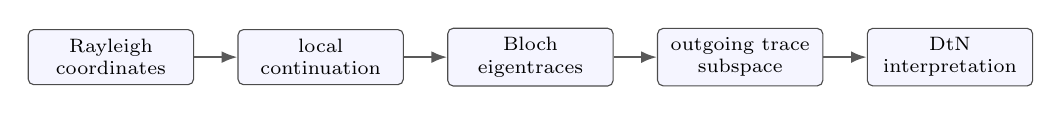
\begin{tikzpicture}[
    node distance=0.55cm,
    box/.style={draw=black!70, rounded corners=2pt, align=center,
      minimum width=2.1cm, minimum height=0.7cm, fill=blue!4,
      font=\scriptsize},
    arrow/.style={-{Latex[length=2mm]}, thick, draw=black!65}
  ]
    \node[box] (rayleigh) {Rayleigh\\coordinates};
    \node[box, right=of rayleigh] (local) {local\\continuation};
    \node[box, right=of local] (bloch) {Bloch\\eigentraces};
    \node[box, right=of bloch] (out) {outgoing trace\\subspace};
    \node[box, right=of out] (dtn) {DtN\\interpretation};
    \draw[arrow] (rayleigh) -- (local);
    \draw[arrow] (local) -- (bloch);
    \draw[arrow] (bloch) -- (out);
    \draw[arrow] (out) -- (dtn);
  \end{tikzpicture}

  \vspace{1em}
  \begin{block}{Central message}
    Rayleigh functions give wall coordinates.  Bloch computations select
    physically admissible trace subspaces of the semi-infinite periodic leads.
  \end{block}
\end{frame}

% Geometry and Cauchy traces are part of the trace-coordinate setup.

\begin{frame}{Reference Cells and Ports}
  \centering
  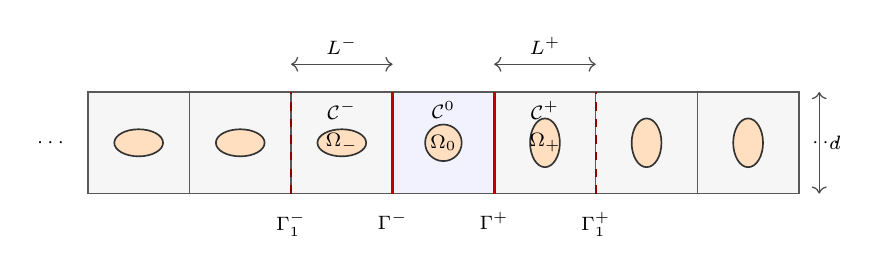
\begin{tikzpicture}[
    x=0.86cm,
    y=0.86cm,
    every node/.style={font=\scriptsize},
    cell/.style={draw=black!65, line width=0.5pt},
    leadcell/.style={fill=gray!7},
    centercell/.style={fill=blue!5},
    inclusion/.style={draw=black!80, fill=orange!25, line width=0.6pt},
    port/.style={draw=red!75!black, line width=1.1pt},
    ghostport/.style={draw=red!55!black, line width=0.75pt, dashed},
    dim/.style={<->, draw=black!70, line width=0.45pt}
  ]
    \foreach \x in {-4.5,-3.0,-1.5} {
      \draw[cell, leadcell] (\x,-0.75) rectangle ++(1.5,1.5);
      \draw[inclusion] (\x+0.75,0) ellipse [x radius=0.36, y radius=0.20];
    }
    \draw[cell, centercell] (0,-0.75) rectangle (1.5,0.75);
    \draw[inclusion] (0.75,0) circle [radius=0.27];
    \foreach \x in {1.5,3.0,4.5} {
      \draw[cell, leadcell] (\x,-0.75) rectangle ++(1.5,1.5);
      \draw[inclusion] (\x+0.75,0) ellipse [x radius=0.22, y radius=0.36];
    }
    \draw[ghostport] (-1.5,-0.75) -- (-1.5,0.75);
    \draw[port] (0,-0.75) -- (0,0.75);
    \draw[port] (1.5,-0.75) -- (1.5,0.75);
    \draw[ghostport] (3.0,-0.75) -- (3.0,0.75);
    \node at (-0.75,0.48) {$\mathcal C^-$};
    \node at (0.75,0.48) {$\mathcal C^0$};
    \node at (2.25,0.48) {$\mathcal C^+$};
    \node[below] at (-1.5,-0.88) {$\Gamma_1^-$};
    \node[below] at (0,-0.88) {$\Gamma^-$};
    \node[below] at (1.5,-0.88) {$\Gamma^+$};
    \node[below] at (3.0,-0.88) {$\Gamma_1^+$};
    \node at (-0.75,0) {$\Omega_-$};
    \node at (0.75,0) {$\Omega_0$};
    \node at (2.25,0) {$\Omega_+$};
    \draw[dim] (-1.5,1.16) -- (0,1.16);
    \node[above] at (-0.75,1.16) {$L^-$};
    \draw[dim] (1.5,1.16) -- (3.0,1.16);
    \node[above] at (2.25,1.16) {$L^+$};
    \draw[dim] (6.3,-0.75) -- (6.3,0.75);
    \node[right] at (6.3,0) {$d$};
    \node[left] at (-4.65,0) {$\cdots$};
    \node[right] at (6.05,0) {$\cdots$};
  \end{tikzpicture}

  \vspace{0.6em}
  \small
  The center inclusion is \(\Omega_0\), with
  \(\Sigma=\partial\Omega_0\).  Port normals are
  \[
    \nu_{\Gamma^-}=-e_x,
    \qquad
    \nu_{\Gamma^+}=+e_x.
  \]
\end{frame}

\begin{frame}{Continuous Cauchy Trace Space}
  For the center ports,
  \[
    \Gamma_0^-=\Gamma^-=\{x=X^-,\;Y^-\le y\le Y^+\},
    \qquad
    \Gamma_0^+=\Gamma^+=\{x=X^+,\;Y^-\le y\le Y^+\}.
  \]
  The natural wall data are Cauchy traces:
  \[
    \tr_{\Gamma^\pm}u
    =
    \begin{bmatrix}
      u|_{\Gamma^\pm}\\
      \partial_{\nu_{\Gamma^\pm}}u|_{\Gamma^\pm}
    \end{bmatrix}
    \in
    H^{1/2}(\Gamma^\pm)\times H^{-1/2}(\Gamma^\pm).
  \]
  \begin{block}{Important}
    Bloch theory acts on wall Cauchy traces, not merely on scalar amplitudes.
  \end{block}
\end{frame}

\begin{frame}{Half-lead Wall Indexing}
  In the positive half-lead,
  \[
    \Gamma_j^+=\Gamma^+ + jL^+e_x,
    \qquad j=0,1,2,\ldots.
  \]
  In the negative half-lead,
  \[
    \Gamma_j^-=\Gamma^- - jL^-e_x,
    \qquad j=0,1,2,\ldots.
  \]
  Thus \(j\) increases away from the center: toward \(+\infty\) in the
  positive lead and toward \(-\infty\) in the negative lead.
  \[
    z_j^\pm=\tr_{\Gamma_j^\pm}u
    =
    \begin{bmatrix}D_j^\pm\\N_j^\pm\end{bmatrix}.
  \]
  \begin{block}{Total trace}
    \(z_j^\pm\) is the \textbf{total trace}; it is \textbf{not an incoming trace}.
    The entries \(D_j^\pm,N_j^\pm\) are Rayleigh-coordinate Cauchy trace
    coefficients.
  \end{block}
\end{frame}

% Rayleigh coordinates are derived before any Bloch-mode selection.

\begin{frame}{From Quasiperiodicity to Fourier Coordinates}
  Assume transverse quasiperiodicity:
  \[
    u(x,y+d)=e^{\ii\beta d}u(x,y).
  \]
  Remove the phase:
  \[
    v(x,y)=e^{-\ii\beta y}u(x,y),
    \qquad
    v(x,y+d)=v(x,y).
  \]
  For each fixed \(x\), expand the periodic function:
  \[
    v(x,y)
    =
    \sum_{m\in\mathbb Z}
    \widehat v_m(x)e^{2\pi\ii my/d}.
  \]
\end{frame}

\begin{frame}{Rayleigh Wall Basis}
  Reinsert the quasiperiodic phase:
  \[
    u(x,y)
    =
    \sum_{m\in\mathbb Z}u_m(x)\psi_m(y),
  \]
  where
  \[
    \psi_m(y)=\frac{1}{\sqrt d}e^{\ii\beta_m y},
    \qquad
    \beta_m=\beta+\frac{2\pi m}{d}.
  \]
  \begin{block}{Interpretation}
    The functions \(\psi_m\) are transverse wall-coordinate functions for
    \(y\)-quasiperiodic traces.
  \end{block}
\end{frame}

\begin{frame}{Homogeneous Rayleigh--Bloch Orders}
  In a homogeneous background,
  \[
    (\Delta+k^2)u=0.
  \]
  Substitution gives one ODE for each order:
  \[
    u_m''(x)+\gamma_m^2u_m(x)=0,
    \qquad
    \gamma_m^2=k^2-\beta_m^2.
  \]
  Hence
  \[
    u_m(x)=a_m e^{\ii\gamma_m x}+b_m e^{-\ii\gamma_m x}.
  \]
  The homogeneous expansion is
  \[
    u(x,y)=
    \sum_m
    \left(
      a_m e^{\ii\gamma_m x}
      +
      b_m e^{-\ii\gamma_m x}
    \right)\psi_m(y).
  \]
\end{frame}

\begin{frame}{Propagation, Evanescence, and Grazing}
  \begin{itemize}
    \item If \(k^2>\beta_m^2\), then \(\gamma_m\) is real:
    the order is propagating.
    \item If \(k^2<\beta_m^2\), write
    \[
      \alpha_m=\sqrt{\beta_m^2-k^2},
      \qquad
      \gamma_m=\ii\alpha_m,
    \]
    so the factors are exponential.
    \item The grazing case \(\gamma_m=0\) is singular and numerically delicate.
  \end{itemize}
  \begin{alertblock}{Terminology}
    These separated waves are homogeneous Rayleigh--Bloch orders.  They are
    not the same as Bloch modes of a periodic lead.
  \end{alertblock}
\end{frame}

% Truncated trace coordinates are still only coordinate data.

\begin{frame}{Truncated Rayleigh Trace Coordinates}
  Truncate to
  \[
    |m|\le M,
    \qquad
    K=2M+1.
  \]
  Dirichlet and Neumann trace coefficients are
  \[
    D,N\in\mathbb C^K,
    \qquad
    \begin{bmatrix}D\\N\end{bmatrix}
    \in
    \mathbb C^K\times\mathbb C^K.
  \]
  \begin{block}{Coordinate space}
    \(\mathbb C^K\times\mathbb C^K\) is a finite coordinate space for Cauchy
    traces, not a physical outgoing condition by itself.
  \end{block}
\end{frame}

\begin{frame}{Rayleigh Coordinates Are Not Periodic-lead Bloch Modes}
  \begin{itemize}
    \item Rayleigh basis functions are wall coordinate functions.
    \item A periodic-lead Bloch mode is a Floquet multiplier eigenmode of a
    one-cell propagation or scattering problem.
    \item A Bloch mode can be spatially complicated inside a lead cell, while
    its wall trace is represented in Rayleigh coordinates.
  \end{itemize}
  \[
    \text{Rayleigh coordinates}
    =
    \text{ambient trace coordinates},
    \qquad
    \text{Bloch modes}
    =
    \text{cell eigentraces}.
  \]
\end{frame}

% Local continuation closes the first conceptual stage.

\begin{frame}{Arbitrary Local Rayleigh Cauchy Data}
  In a homogeneous port strip, arbitrary truncated Cauchy data can be locally
  continued.  At a reference wall \(x=X_L\),
  \[
    D=a+b,
    \qquad
    N=\ii\Gamma(a-b),
    \qquad
    \Gamma=\operatorname{diag}(\gamma_m).
  \]
  If \(\Gamma\) is invertible,
  \[
    a=\frac12\left(D+(\ii\Gamma)^{-1}N\right),
    \qquad
    b=\frac12\left(D-(\ii\Gamma)^{-1}N\right).
  \]
  The local field is
  \[
    u(x,y)=
    \sum_m a_m e^{\ii\gamma_m(x-X_L)}\psi_m(y)
    +
    \sum_m b_m e^{-\ii\gamma_m(x-X_L)}\psi_m(y).
  \]
\end{frame}

\begin{frame}{Local Continuation Is Not Radiation}
  \begin{block}{What local continuation says}
    A Cauchy trace can be extended through a homogeneous neighborhood of the
    wall by Rayleigh orders.
  \end{block}
  \begin{alertblock}{What it does not say}
    The trace may still be non-admissible for the semi-infinite exterior.
    Radiation/admissibility is a condition at infinity, not a local algebraic
    decomposition into \(a\) and \(b\).
  \end{alertblock}
  This is the distinction between a coordinate section and a transparent
  exterior boundary condition.
\end{frame}

\section{Bloch Propagation and Radiation Selection}

\begin{frame}{Total-Trace Extension}
  \[
    z_j^\pm=\tr_{\Gamma_j^\pm}u
  \]
  is the \textbf{total trace} on the wall, \textbf{not an incoming trace}.
  For a positive periodic lead,
  \[
    z_{j+1}^+ = P^+ z_j^+,
    \qquad
    z_j^+=(P^+)^jz_0^+.
  \]
  If \(P^-\) is still defined by a left-to-right cell convention, then moving
  away from the center in the negative lead uses the inverse iteration:
  \[
    z_j^-=(P^-)^{-j}z_0^-,
    \qquad j=0,1,2,\ldots.
  \]
  Here \(P^\pm\) propagates the \textbf{total trace} through one periodic lead
  cell.
\end{frame}

\begin{frame}{Why Radiation Is Not Optional}
  Given an arbitrary nonzero \textbf{total trace} at the center port, one can
  formally define
  \[
    z_j^+=(P^+)^jz_0^+,
    \qquad
    z_j^-=(P^-)^{-j}z_0^-.
  \]
  This gives a cell-by-cell \emph{local continuation}, but it may contain growing
  or propagating components at infinity.
  \[
    \text{admissibility:}\qquad
    z_0^+\in E_{\mathrm{out}}^+,
    \qquad
    z_0^-\in E_{\mathrm{out}}^-.
  \]
  Schematically, for a center-cell map \(P^0\),
  \[
    z_0^-\in E_{\mathrm{out}}^-,
    \qquad
    P^0z_0^-\in E_{\mathrm{out}}^+.
  \]
  \begin{alertblock}{Role of the outgoing subspaces}
    They do not make extension possible.  They select the physically
    admissible extensions at infinity.
  \end{alertblock}
\end{frame}

\begin{frame}{Non-periodic Chains and Bloch Eigentraces}
  For a non-periodic chain, \(P_j\) is the propagation operator through the
  \(j\)-th cell:
  \[
    z_{j+1}=P_jz_j,
    \qquad
    z_N=P_{N-1}\cdots P_1P_0z_0.
  \]
  In a periodic lead, the same one-cell map is reused:
  \[
    P_j=P,
    \qquad
    Pz=\lambda z,
    \qquad
    z_N=\lambda^Nz.
  \]
  \begin{block}{Why periodicity matters}
    A local cell eigenproblem can be written even for a defect cell, but
    \emph{radiation/admissibility} becomes meaningful only after specifying the
    infinite exterior structure.
  \end{block}
\end{frame}

\begin{frame}{One-cell Scattering Experiments}
  \footnotesize
  One-cell experiments construct scattering blocks:
  \[
    \begin{bmatrix}b^L\\ a^R\end{bmatrix}
    =
    \begin{bmatrix}
      R_L & T_{R\to L}\\
      T_{L\to R} & R_R
    \end{bmatrix}
    \begin{bmatrix}a^L\\ b^R\end{bmatrix}.
  \]
  These experiments use one-sided inputs such as
  \((a^L,b^R)=(a^L,0)\), but they are not the objects propagated through the
  infinite lead.  If \(b^R=0\), then
  \[
    b^L=R_La^L,
    \qquad
    a^R=T_{L\to R}a^L,
  \]
  so the left-wall \textbf{total directional state} is
  \[
    \begin{bmatrix}a^L\\b^L\end{bmatrix}
    =
    \begin{bmatrix}a^L\\R_La^L\end{bmatrix},
    \qquad
    \text{not }
    \begin{bmatrix}a^L\\0\end{bmatrix}.
  \]
  \begin{block}{Remark}
    If \(\begin{bmatrix}a^L\\0\end{bmatrix}\) is forced into \(P\) as a
    \textbf{total directional state}, it is only a formal Cauchy continuation;
    the next wall generally has both directional components.
  \end{block}
\end{frame}

\begin{frame}{Propagation Map from Scattering Blocks}
  \footnotesize
  If \(T_{R\to L}\) is invertible, then
  \[
    b^R=T_{R\to L}^{-1}(b^L-R_La^L),
  \]
  and hence
  \[
    \begin{bmatrix}a^R\\b^R\end{bmatrix}
    =
    P
    \begin{bmatrix}a^L\\b^L\end{bmatrix},
  \]
  where \(\begin{bmatrix}a^L\\b^L\end{bmatrix}\) and
  \(\begin{bmatrix}a^R\\b^R\end{bmatrix}\) are \textbf{total directional
  states} on the left and right walls of one cell.
  The block formula is
  \[
    P=
    \begin{bmatrix}
      T_{L\to R}-R_RT_{R\to L}^{-1}R_L
      &
      R_RT_{R\to L}^{-1}
      \\
      -T_{R\to L}^{-1}R_L
      &
      T_{R\to L}^{-1}
    \end{bmatrix}.
  \]
  This formula only illustrates that propagation acts on the
  \textbf{total directional state}.  Numerically, one may still use
  \[
    A_{\mathrm{sc}}z=\lambda B_{\mathrm{sc}}z
  \]
  without explicitly inverting \(T_{R\to L}\).
\end{frame}

\begin{frame}{Reconstructing the Field Inside a Cell}
  \footnotesize
  For one generic lead cell, \(P\) propagates wall \textbf{total directional
  states}.  To recover the field inside the cell, return to the
  \emph{local cell problem}.
  \[
    \begin{bmatrix}b^L\\a^R\end{bmatrix}
    =
    \begin{bmatrix}R_L&T_{R\to L}\\T_{L\to R}&R_R\end{bmatrix}
    \begin{bmatrix}a^L\\b^R\end{bmatrix}.
  \]
  Given
  \[
    z^L=\begin{bmatrix}a^L\\b^L\end{bmatrix},
    \qquad
    b^R=T_{R\to L}^{-1}(b^L-R_La^L),
  \]
  the cell field is the two-sided scattering response driven by
  \((a^L,b^R)\).  With
  \(\psi_m(y)=d^{-1/2}e^{\ii\beta_m y}\) and
  \(\gamma_m^2=k^2-\beta_m^2\),
  \[
    u_{\mathrm{inc}}^L
    =
    \sum_m a_m^L e^{\ii\gamma_m(x-X_L)}\psi_m(y),
    \qquad
    u_{\mathrm{inc}}^R
    =
    \sum_m b_m^R e^{-\ii\gamma_m(x-X_R)}\psi_m(y).
  \]
  The basis experiments \([a^L;0]\) and \([0;b^R]\) build the cell response;
  a general \textbf{total trace} uses their linear combination.
  \begin{block}{Reconstruction principle}
    Wall traces determine the cell field through the \emph{local cell problem}.
  \end{block}
\end{frame}

% Incoming/outgoing trace subspaces are selected by the lead propagation.

\begin{frame}{Mode Selection by Multipliers}
  Assume \(\lambda^\pm\) propagates one cell from left to right in the
  corresponding reference lead.
  For a positive half-lead,
  \[
    \boxed{
    \text{decay toward }+\infty
    \iff
    |\lambda^+|<1.
    }
  \]
  For a negative half-lead, using the same left-to-right convention,
  \[
    \boxed{
    \text{decay toward }-\infty
    \iff
    |\lambda^-|>1.
    }
  \]
  \begin{alertblock}{Unit-circle caveat}
    For real-frequency propagating modes with \(|\lambda^\pm|=1\), incoming versus
    outgoing needs limiting absorption, flux, or group velocity, not modulus
    alone.
  \end{alertblock}
\end{frame}

\begin{frame}{Selected Trace Subspaces}
  \small
  At the continuous level, the admissible trace spaces are true subspaces:
  \[
    \mathcal E_{\mathrm{in}}^\pm,
    \mathcal E_{\mathrm{out}}^\pm
    \subset
    H^{1/2}(\Gamma^\pm)\times H^{-1/2}(\Gamma^\pm).
  \]
  After Rayleigh truncation to \(|m|\le M\), \(K=2M+1\), the selected
  eigentraces are stored as trace basis matrices:
  \[
    D_{\mathrm{in}}^\pm,N_{\mathrm{in}}^\pm
    \in\mathbb C^{K\times K_{\mathrm{in}}^\pm},
    \qquad
    D_{\mathrm{out}}^\pm,N_{\mathrm{out}}^\pm
    \in\mathbb C^{K\times K_{\mathrm{out}}^\pm}.
  \]
  Here \(K_{\mathrm{out}}^\pm\) is the number of outgoing Bloch eigentraces
  retained at \(\Gamma^\pm\); \(K_{\mathrm{in}}^\pm\) is defined similarly.
  Thus
  \[
    E_{\mathrm{in/out}}^\pm
    =
    \range
    \begin{bmatrix}
      D_{\mathrm{in/out}}^\pm\\
      N_{\mathrm{in/out}}^\pm
    \end{bmatrix}
    \subset
    \mathbb C^K\times\mathbb C^K.
  \]
\end{frame}

\begin{frame}{Incoming Wave Versus One Bloch Mode}
  A legal incoming trace is generally a linear combination:
  \[
    \begin{bmatrix}
      D_{\mathrm{in}}^\pm\\
      N_{\mathrm{in}}^\pm
    \end{bmatrix}
    p_{\mathrm{in}}^\pm.
  \]
  Here \(p_{\mathrm{in}}^\pm\in\mathbb C^{K_{\mathrm{in}}^\pm}\); an outgoing
  scattered coefficient vector would satisfy
  \(r^\pm\in\mathbb C^{K_{\mathrm{out}}^\pm}\).

  It is a single Bloch mode only if \(p_{\mathrm{in}}^\pm\) selects one
  eigenvector column.
  \begin{block}{Do not overuse ``Bloch mode''}
    An arbitrary incoming wave is an element of the incoming Bloch trace
    subspace, not necessarily one Bloch mode.
  \end{block}
\end{frame}

\section{DtN Interpretation and Joly--Fliss Comparison}

\begin{frame}{Classical DtN Graph Form}
  Classical transparent boundary conditions are often written as a DtN graph:
  \[
    N=\Lambda_{\mathrm{out}}D,
    \qquad
    \Lambda_{\mathrm{out}}:
    H^{1/2}(\Gamma^\pm)\to H^{-1/2}(\Gamma^\pm).
  \]
  In left/right port notation one may write schematically
  \[
    \pm\partial_x u+\Lambda^\pm u=0
    \quad\text{on }\Gamma^\pm.
  \]
  This is a graph relation between Dirichlet and Neumann traces:
  \[
    D\mapsto N.
  \]
  \begin{alertblock}{Branch selection}
    Such a map is meaningful only after selecting the outgoing/admissible
    exterior branch.
  \end{alertblock}
\end{frame}

\begin{frame}{Cauchy Trace-subspace Form}
  At the continuous level, our port condition is
  \[
    \begin{bmatrix}D\\N\end{bmatrix}
    \in
    \mathcal E_{\mathrm{out}}^\pm.
  \]
  After truncation, the corresponding discrete condition is
  \[
    \begin{bmatrix}D\\N\end{bmatrix}
    \in
    E_{\mathrm{out}}^\pm.
  \]
  If \(D_{\mathrm{out}}\) is square and invertible, the discrete condition can
  be written as a DtN graph:
  \[
    D=D_{\mathrm{out}}a,
    \qquad
    N=N_{\mathrm{out}}a
    \quad\Longrightarrow\quad
    N=N_{\mathrm{out}}D_{\mathrm{out}}^{-1}D.
  \]
  \begin{block}{Graph representation}
    A DtN map is a graph representation of an outgoing Cauchy trace subspace.
  \end{block}
\end{frame}

\begin{frame}{Why Keep the Subspace?}
  In practice, \(D_{\mathrm{out}}\) may be rectangular, rank-deficient, or
  ill-conditioned.  The discrete Cauchy trace subspace remains meaningful:
  \[
    \begin{bmatrix}D\\N\end{bmatrix}
    =
    \begin{bmatrix}
      D_{\mathrm{out}}\\
      N_{\mathrm{out}}
    \end{bmatrix}a.
  \]
  \[
    \boxed{
      \text{Use the outgoing Cauchy subspace directly instead of forcing a DtN map.}
    }
  \]
  This is the port-trace version of a DtN transparent boundary condition.
\end{frame}

% Joly--Fliss comparison belongs to the DtN-interpretation stage.

\begin{frame}{Joly--Fliss Route}
  A schematic view of the absorbing half-guide construction is
  \[
    \text{absorbing half-guide problem}
    \Longrightarrow
    \text{admissible branch}
  \]
  \[
    \Longrightarrow
    R_\varepsilon^\pm,\ S_\varepsilon^\pm,\ \Lambda_\varepsilon^\pm
    \Longrightarrow
    \text{extension}.
  \]
  \begin{block}{Interpretation}
    The absorption / limiting absorption selects a half-guide solution and
    the associated transparent boundary operators.
  \end{block}
  Fixed absorption is a regularization device, not the final lossless
  eigenvalue condition.
\end{frame}

\begin{frame}{What Is Different Here?}
  Joly--Fliss extension operators are tied to the admissible half-guide
  problem.  They are not separate explicit continuation formulas for arbitrary
  non-admissible Cauchy traces.

  \vspace{0.6em}
  Our route is
  \[
    \text{arbitrary total trace}
    \Longrightarrow
    \text{local / periodic-cell extension}
  \]
  \[
    \Longrightarrow
    \text{Bloch multiplier selection}
    \Longrightarrow
    E_{\mathrm{out}}^\pm.
  \]
  \begin{alertblock}{Key distinction}
    Local continuability does not imply radiation admissibility.
  \end{alertblock}
\end{frame}

\section{Consequences for Scattering and TEP Formulations}

\begin{frame}{Forced Lead Scattering}
  In a forced scattering problem,
  \[
    u=u_{\mathrm{in}}+u_s.
  \]
  In truncated Rayleigh coordinates, the total port trace is incoming plus
  outgoing:
  \[
    \begin{bmatrix}
      D^\pm\\
      N^\pm
    \end{bmatrix}
    =
    \begin{bmatrix}
      D_{\mathrm{in}}^\pm\\
      N_{\mathrm{in}}^\pm
    \end{bmatrix}p_{\mathrm{in}}^\pm
    +
    \begin{bmatrix}
      D_{\mathrm{out}}^\pm\\
      N_{\mathrm{out}}^\pm
    \end{bmatrix}r^\pm.
  \]
  Only the scattered part is outgoing/admissible.
\end{frame}

\begin{frame}{Eigenvalue / TEP-type Problem}
  In an eigenvalue formulation, there is no prescribed incoming forcing.
  At the continuous level, the total trace must satisfy
  \[
    \tr_{\Gamma^\pm}u
    \in
    \mathcal E_{\mathrm{out}}^\pm.
  \]
  In the truncated computation this is represented by membership in
  \(E_{\mathrm{out}}^\pm\).
  The numerical target is a nontrivial solution of a homogeneous admissible
  system:
  \[
    \mathcal A(k,\beta)x=0.
  \]
  \begin{block}{Shared machinery}
    Forced scattering and eigenvalue searches use the same trace spaces; the
    right-hand side and numerical target are different.
  \end{block}
\end{frame}

% Caveats and summary close the consequences section.

\begin{frame}{Numerical and Conceptual Caveats}
  \begin{itemize}
    \item Rayleigh truncation is a finite-dimensional approximation.
    \item Grazing orders \(\gamma_m=0\) are singular or ill-conditioned.
    \item Outgoing Bloch trace is not the same as local right-going Rayleigh
    amplitude.
    \item Non-periodic exterior chains require infinite products, not one-cell
    multiplier selection.
    \item DtN graph form may fail or be ill-conditioned; Cauchy trace
    subspace form can remain meaningful.
  \end{itemize}
\end{frame}

\begin{frame}{Takeaway}
  \begin{enumerate}
    \item Rayleigh functions give wall trace coordinates.
    \item Bloch eigentraces come from one-cell periodic propagation.
    \item Radiation/admissibility selects incoming and outgoing half-lead
    trace subspaces.
    \item DtN maps are graph representations of those subspaces when such
    graphs are well behaved.
  \end{enumerate}
  \[
    \boxed{\text{The port condition is the exterior radiation condition compressed to }\Gamma^\pm.}
  \]
\end{frame}

\end{document}
